%!TEX TS-program = pdflatexmk

% Copyright (c) 2018 - 2022, Martin Scheidt (ISC license)
% Permission to use, copy, modify, and/or distribute this file for any purpose with or without fee is hereby granted, provided that the above copyright notice and this permission notice appear in all copies.

\documentclass[tikz,border=2]{standalone}
\usepackage{tikz-trackschematic} % loading the library

\begin{document}
  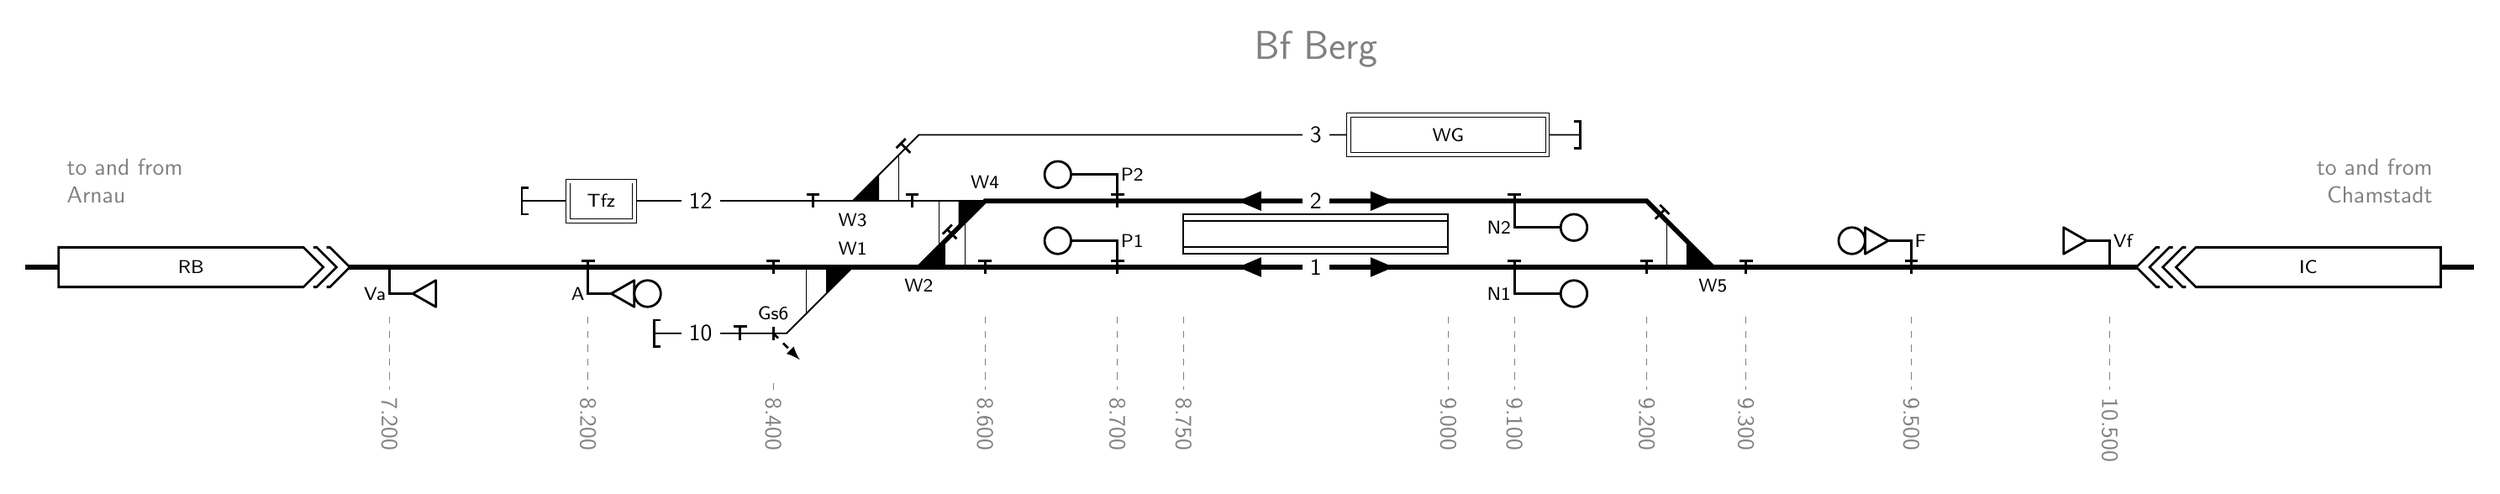
\begin{tikzpicture}[font=\sffamily]
  { % station names
    \tikzset{every node/.style={foreground!50!background}};
    \node[right,align=left] at ( 2,1.3) {to and from\\ Arnau};
    \node                   at (21,3.3) {{\LARGE Bf Berg}};
    \node[left,align=right] at (38,1.3) {to and from\\ Chamstadt};
  }
  % coordinates
  \coordinate (A)  at ( 1.5, 0);
  \coordinate (B)  at (38.5, 0);

  \coordinate (E1) at ( 9  , 1);
  \coordinate (E2) at (11  ,-1);
  \coordinate (E3) at (25  , 2);
  \coordinate (H1) at (15  , 2);
  \coordinate (H2) at (26  , 1);

  \coordinate (Y1) at (14  , 0);
  \coordinate (Y2) at (15  , 0);
  \coordinate (Y3) at (14  , 1);
  \coordinate (Y4) at (16  , 1);
  \coordinate (Y5) at (27  , 0);
  \coordinate (Y6) at (12.8,-1);

  \coordinate (S1) at ( 7  , 0);
  \coordinate (S2) at (10  , 0);
  \coordinate (S3) at (18  , 0);
  \coordinate (S4) at (18  , 1);
  \coordinate (S5) at (24  , 0);
  \coordinate (S6) at (24  , 1);
  \coordinate (S7) at (30  , 0);
  \coordinate (S8) at (33  , 0);

  \coordinate (T1) at ( 6  , 0);
  \coordinate (T2) at (10.2, 1);
  \coordinate (T3) at (23  , 2);
  \coordinate (T4) at (34  , 0);

  \coordinate (P1) at (21  , 0);
  \coordinate (P2) at (21  , 1);

  \coordinate (HM) at (0,-1.85);

  { %% topology
    % tracks
    \maintrack (A) -- (B);
    \maintrack (Y2) -- (Y4) -- (H2) -- (Y5);
    \secondarytrack (E1) -- (Y4);
    \secondarytrack (E2) -- ++( 2,0) -- (Y1);
    \secondarytrack (Y3) -- (H1) -- (E3);

    % track numbers
    \tracklabel at (11.7, 1) label (12);
    \tracklabel at (11.7,-1) label (10);
    \tracklabel at (21  , 2) label (3);
    \tracklabel at (P2) label (2);
    \tracklabel at (P1) label (1);

    % bufferstops
    \bufferstop[backward] at (E1);
    \bufferstop[backward] at (E2);
    \bufferstop[forward]  at (E3);

    % turnouts
    \tikzset{every node/.style={fouling point}};
    \turnout[backward,branch=right] at (Y1) label (W1);
    \turnout[forward ,branch=left ] at (Y2) label (W2);
    \turnout[forward ,branch=left ] at (Y3) label (W3);
    \turnout[backward,branch=right] at (Y4) label (W4);
    \turnout[backward,branch=left ] at (Y5) label (W5);
    \derailer[forward,branch=right] at (Y6) label (Gs6);
  }
  { %% traffic control
    % signals
    \distantsignal[forward]  at (S1) label (Va);

    \signal[distant,route,forward] at (S2) label (A);

    \routesignal[backward]   at (S3) label (P1);
    \routesignal[backward]   at (S4) label (P2);

    \routesignal[forward]    at (S5) label (N1);
    \routesignal[forward]    at (S6) label (N2);

    \signal[distant,route,backward] at (S7) label (F);

    \distantsignal[backward] at (S8) label (Vf);
    
    % routes
    \route[backward] at (20,0);
    \route[forward]  at (22,0);
    \route[backward] at (20,1);
    \route[forward]  at (22,1);

    % clearing points
    \tikzset{every node/.style={backward}};
    \clearingpoint[] at (10  , 0) label ();
    \clearingpoint[] at (12.3,-1) label ();
    \clearingpoint[] at (12.8, 0) label ();
    \clearingpoint[] at (13.4, 1) label ();
    \clearingpoint[] at (14.9, 1) label ();
    \coordinate (H3) at ($(Y2)!0.5!(Y4)$); % using tikz calc library
    \clearingpoint[rotate=45] at (H3) label ();
    \coordinate (H4) at ($(Y3)!0.8!(H1)$); % using tikz calc library
    \clearingpoint[rotate=45] at (H4) label ();
    \clearingpoint[] at (16  , 0) label ();
    \clearingpoint[] at (18  , 1) label ();
    \clearingpoint[] at (18  , 0) label ();
    \clearingpoint[] at (24  , 1) label ();
    \clearingpoint[] at (24  , 0) label ();
    \clearingpoint[] at (26  , 0) label ();
    \clearingpoint[] at (27.5, 0) label ();
    \coordinate (H5) at ($(Y5)!0.8!(H2)$); % using tikz calc library
    \clearingpoint[rotate=315] at (H5) label ();
    \clearingpoint[] at (30  , 0) label ();
  }
  { %% vehicles
    \train[run=normal,forward] at (T1) label (RB);
    \train[run=fast,backward]  at (T4) label (IC);
    \parkedvehicles[length=3cm] at (T3) label (WG);
    \parkedvehicles[length=1cm] at (T2) label (Tfz);
  }
  { %% constructions
    % platforms
    \platform[side=right] at (P2);
    \platform[side=left ] at (P1);
  }
  { %% measures
    % hectometer posts
    \tikzset{hectometer base={(HM)},orientation=right};
    \hectometer[] at (S1)      label ( 7.200);
    \hectometer[] at (S2)      label ( 8.200);
    \hectometer[] at (12.8,-1) label ( 8.400);
    \hectometer[] at (16  , 0) label ( 8.600);
    \hectometer[] at (S3)      label ( 8.700);
    \hectometer[] at (19  , 0) label ( 8.750);
    \hectometer[] at (23  , 0) label ( 9.000);
    \hectometer[] at (S5)      label ( 9.100);
    \hectometer[] at (26  , 0) label ( 9.200);
    \hectometer[] at (27.5, 0) label ( 9.300);
    \hectometer[] at (S7)      label ( 9.500);
    \hectometer[] at (S8)      label (10.500);
  }
  \end{tikzpicture}
\end{document}